\documentclass[aspectratio=169,12pt]{beamer}
\usetheme{Madrid}
\usecolortheme{dolphin}
\usefonttheme{professionalfonts}
\setbeamertemplate{navigation symbols}{}
\setbeamertemplate{footline}{}

\usepackage[T1]{fontenc}
\usepackage[utf8]{inputenc}
\usepackage{graphicx}
\usepackage{amsmath,amssymb}
\usepackage{hyperref}
\usepackage{siunitx}
\usepackage{physics}
\usepackage{tikz}
\usetikzlibrary{angles,quotes}

\begin{document}

\begin{frame}{Le Qubit dans tout ses états}
    \begin{columns}[T]
    \begin{column}{0.49\textwidth}
      \begin{center}
      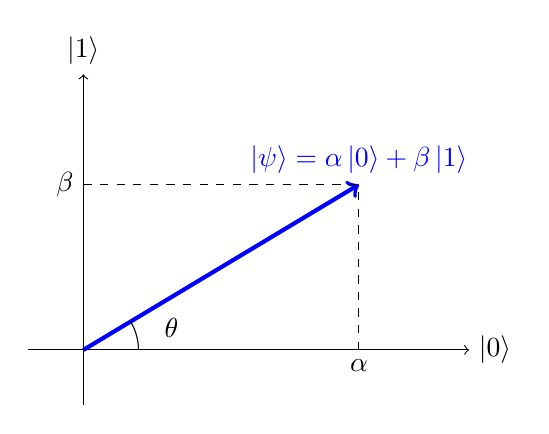
\begin{tikzpicture}[scale=1.4]
        \draw[->] (-0.5,0) -- (3.5,0) node[right] {$\ket{0}$};
        \draw[->] (0,-0.5) -- (0,2.5) node[above] {$\ket{1}$};
        \draw[->,thick,blue,line width=1.5pt] (0,0) -- (2.5,1.5) node[above] {$\ket{\psi} = \alpha\ket{0} + \beta\ket{1}$};
        \draw[dashed] (2.5,0) node[below] {$\alpha$} -- (2.5,1.5);
        \draw[dashed] (0,1.5) node[left] {$\beta$} -- (2.5,1.5);
        \draw (0.5,0) arc (0:31:0.5);
        \node at (0.8,0.2) {$\theta$};
      \end{tikzpicture}
      \end{center}
    \end{column}
    \begin{column}{0.49\textwidth}
    \begin{itemize}
        \item Nous avions jusqu'à présent décrit le qubit comme une superposition linéaire d'états sans trop préciser la nature des coefficients $\alpha$ et $\beta$.
        \begin{equation*}
            \ket{\psi} = \alpha \ket{0} + \beta \ket{1}
        \end{equation*}
        \item La condition de normalisation impose:
        \begin{equation*}
            1 = |\alpha|^{2} + |\beta|^{2}
        \end{equation*}
        \item Avec des nombres réels, on a:
        \begin{equation*}
            \alpha = \cos(\theta) \qquad \beta = \sin(\theta)
        \end{equation*} 
    \end{itemize}
    \end{column}
    \end{columns}
\end{frame}

\begin{frame}{Le Qubit dans tout ses états}
    \begin{itemize}
        \item En réalité, ces coefficient peuvent posséder des phases complexes:
        \begin{equation*}
            \ket{\psi} = \alpha e^{i\phi_A} \ket{0} + \beta e^{i\phi_B} \ket{1}
        \end{equation*}
        \item Comme les états quantiques sont identiques à une constante multiplicative près, nous pouvons choisir de faire disparaitre la phase globale $e^{i\phi_A}$:
        \begin{equation*}
            \ket{\psi} = \alpha \ket{0} + e^{i\phi_B - \phi_A}\beta \ket{1}
        \end{equation*}
        \item L'expression générale d'un qubit est donc:
        \begin{equation*}
            \ket{\psi} = \cos\left(\frac{\theta}{2}\right) \ket{0} + e^{i\phi}\sin\left(\frac{\theta}{2}\right) \ket{1}
        \end{equation*}
    \end{itemize}
\end{frame}

\begin{frame}{Le Qubit dans tout ses états}
    \begin{columns}[T]
    \begin{column}{0.35\textwidth}
      \begin{center}
      \includegraphics{../../figures/bloch.png}
      \end{center}
    \end{column}
    \begin{column}{0.64\textwidth}
        \begin{itemize}
            \item La convention est de noter l'état général d'un qubit comme:
            \begin{equation*}
            \boxed{
                \ket{\psi} = \cos\left(\frac{\theta}{2}\right) \ket{0} + e^{i\phi}\sin\left(\frac{\theta}{2}\right) \ket{1}
            }
            \end{equation*}
            \\~\\~
            \item En raison de la visualisation sur la \textit{sphère de Bloch}.
        \end{itemize}
    \end{column}
    \end{columns}
\end{frame}

\begin{frame}{Conséquences pour les vecteurs "bra"}
    \begin{itemize}
        \item Si un qubit s'écrit maintenant avec des nombres complexes $\alpha,\beta\in\mathbb{C}$:
        \begin{equation*}
            \ket{\psi} = \alpha \ket{0} + \beta \ket{1}
        \end{equation*}

        %\vspace{5mm}
        \item Alors le "bra" doit s'écrire avec les coefficient complexes conjugés:
        \begin{equation*}
            \bra{\psi} = \alpha^* \bra{0} + \beta^* \bra{1}
        \end{equation*}

        %\vspace{5mm}
        \item De telle manière à conserver un nombre réel pour la norme: 
        \begin{align*}
            1 = \braket{\psi}{\psi} 
            &= \alpha^*\alpha \braket{0}{0} + \beta^*\beta \braket{1}{1} \\ 
            %&= \alpha^*\alpha + \beta^*\beta \\
            &= |\alpha|^2 + |\beta|^2
        \end{align*}
    \end{itemize}
\end{frame}

\begin{frame}{Conséquences pour les matrices}
    \begin{itemize}   
        \item En ce qui concerne les matrices,
        \begin{equation*}
            U \ket{\psi} = \ket{\psi'} \quad\leftrightarrow\quad 
            \begin{pmatrix}
                a & b \\
                c & d
            \end{pmatrix}
            \begin{pmatrix}
                \alpha \\
                \beta
            \end{pmatrix}
             =
            \begin{pmatrix}
                a\alpha + b\beta \\
                c\alpha + d\beta
            \end{pmatrix}
        \end{equation*}

        %\vspace{5mm}
        \item Il est nécessaire que la matrice reproduisant l'opération sur le "bra" ait également des coefficients conjugués, en plus d'être inversés par rapport à la diagonale:
        \begin{equation*}
            \bra{\psi} U^\dagger = \bra{\psi'} \quad\leftrightarrow\quad 
            \begin{pmatrix}
                \alpha^* & \beta^*
            \end{pmatrix}
            \begin{pmatrix}
                a^* & c^* \\
                b^* & d^*
            \end{pmatrix}
            =
            \begin{pmatrix}
                a^*\alpha^* + b^*\beta^* & c^*\alpha^* + d^*\beta^*
            \end{pmatrix}
        \end{equation*}

        %\vspace{5mm}
        \item Enfin, pour que les opérations quantiques préservent la distinction entre les états, il faut que les matrices associées préservent la condition suivante, dite d'\textit{unitarité}: 
        \begin{equation*}
            \braket{\phi}{\psi} = \bra{\phi} U^\dagger U \ket{\psi} \quad\iff\quad U^\dagger U = I
            =
            \begin{pmatrix}
                1 & 0 \\
                0 & 1
            \end{pmatrix}
        \end{equation*}
    \end{itemize}
\end{frame}

% Version more suitable for an exercise
\begin{frame}{No-Cloning$^*$}
    \begin{itemize}
        \item Supposons qu'une opération $U$ existe pour copier des états génériques $|\phi \rangle$ et $|\psi \rangle$:
        \begin{align*}
            U(|\phi \rangle _{A}|e\rangle _{B}) &= e^{i\alpha (\phi ,e)}|\phi \rangle _{A}|\phi \rangle _{B} \\
            U(|\psi \rangle _{A}|e\rangle _{B}) &= e^{i\alpha (\psi ,e)}|\psi \rangle _{A}|\psi \rangle _{B}
        \end{align*}
        \item Le calcul du produit scalaire des états clonés mène à deux résultats contradictoires:
        \begin{align*}
            | \langle \phi|_{A}\langle e|_{B} \, U^\dagger U \, |\psi \rangle _{A}|e\rangle _{B} | &= | \langle \phi |\psi \rangle |^{2} \\
            | \langle \phi|_{A}\langle e|_{B} \, U^\dagger U \, |\psi \rangle _{A}|e\rangle _{B} | &= | \langle \phi |\psi \rangle |
        \end{align*}
        \item Cela implique que $|\langle \phi |\psi \rangle |=1$ ou $|\langle \phi |\psi \rangle |=0$, en contradiction avec l'hypothèse de généralité des états $|\phi \rangle$ et $|\psi \rangle$.
    \end{itemize}
\end{frame}

% Detailed version
\begin{frame}{No-Cloning}
    \begin{itemize}
        \item Supposons qu'une opération $U$ existe pour copier des états génériques $|\phi \rangle$ et $|\psi \rangle$:
        \begin{align*}
            U(|\phi \rangle _{A}|e\rangle _{B}) &= e^{i\alpha (\phi ,e)}|\phi \rangle _{A}|\phi \rangle _{B} \\
            U(|\psi \rangle _{A}|e\rangle _{B}) &= e^{i\alpha (\psi ,e)}|\psi \rangle _{A}|\psi \rangle _{B}
        \end{align*}
        \item En prenant le produit scalaire des deux états clonés, on obtient:
        \begin{align*}
            \langle \phi|_{A}\langle e|_{B} \, U^\dagger U \, |\psi \rangle _{A}|e\rangle _{B} &= e^{i\alpha (\psi ,e)-i\alpha (\phi ,e)}\langle \phi |\psi \rangle ^{2} \\
            \langle \phi|_{A}\langle e|_{B} \, U^\dagger U \, |\psi \rangle _{A}|e\rangle _{B} &= \langle \phi |\psi \rangle \langle e |e \rangle
        \end{align*}
        \item Mais alors $|\langle \phi |\psi \rangle| = |\langle \phi |\psi \rangle|^{2}$, ce qui implique que $|\langle \phi |\psi \rangle |=1$ ou $|\langle \phi |\psi \rangle |=0$, en contradiction avec l'hypothèse de généralité des états $|\phi \rangle$ et $|\psi \rangle$.
    \end{itemize}
\end{frame}

\begin{frame}{Portes logiques complexes}
    \begin{itemize}
        \item Les nombres complexes nous permettent de définir un nombre beaucoup plus grand d'opérations sur le Qubit
        \item En particulier, il est possible de définir des matrices racines:
        \begin{align*}
            \sqrt{Z} = 
            \begin{pmatrix}
                1 & 0 \\
                0 & i 
            \end{pmatrix}
            &\qquad \longrightarrow \qquad
            (\sqrt{Z})^2 = Z = 
            \begin{pmatrix}
                1 & 0 \\
                0 & -1 
            \end{pmatrix}
            \\
        %\end{align*}
        %\begin{align*}
            \sqrt{X} = \frac{1}{2} 
            \begin{pmatrix}
                1+i & 1-i \\
                1-i & 1+i 
            \end{pmatrix}
            &\qquad \longrightarrow \qquad
            (\sqrt{X})^2 = X =
            \begin{pmatrix}
                0 & 1 \\
                1 & 0  
            \end{pmatrix}
            \\
        \end{align*}
        \item Les portes $X$ et $Z$ font tourner le Qubit sur la sphère de Bloch, et les matrices racines effectuent la moitié de ces rotations.
    \end{itemize}
\end{frame}

\end{document}
